\documentclass[a4paper,12pt]{article}
\usepackage[margin=1in]{geometry}

\usepackage[T2A]{fontenc}			% кодировка
\usepackage[utf8]{inputenc}			% кодировка исходного текста
\usepackage[english,russian]{babel}	% локализация и переносы
\usepackage{graphicx}                % Математика
\usepackage{amsmath,amsfonts,amssymb,amsthm,mathtools} 
\usepackage{mathtext}
\usepackage[T2A]{fontenc}
\usepackage[utf8]{inputenc}

\usepackage{wasysym}

%Заговолок
\author{Бичина Марина 
группа Б04-005 1 курса ФЭФМ}
\title{}
\date{}


\begin{document} % начало документа

\begin{center}
\begin{Large}
{Бичина Марина, Карташов Константин Б04-005, Лабораторная работа №. 5.1.1 <<Экспериментальная проверка уравнения Эйнштейна для фотоэффекта и определение постоянной Планка>>}
\end{Large}
\end{center}
\paragraph{Цель работы:} 
\begin{enumerate}
\itemsep0em
\item Исследовать зависимость фототока от 
\begin{enumerate}
\itemsep0em
\item величины задерживающего потенциала
\item частоты падающего излучения
\end{enumerate}
\item вычислить постоянную Планка
\end{enumerate}

\paragraph{Теоретическая справка:}
\paragraph{}
\textbf{Фотоэффект} -- явление испускания электронов фотокатодом, облучаемым светом. Это явление хорошо объясняется фотонной теорией света: взаимодействие монохроматического света с веществом можно описывать как взаимодействие с веществом частиц, называемых фотонами, которые обладают энергией $ \hbar \omega $ и импульсом $ \hbar\omega/c $. При столкновении фотона с электроном фотокатода энергия фотона полностью передается электрону, и фотон прекращает свое существование. Энергетический баланс этого взаимодействия для вылетающих электронов описывается уравнением
	
\begin{equation}
\hbar \omega = E_{max} + W
\label{energy balance}
\end{equation}
	
\begin{figure}[h!]
\centering
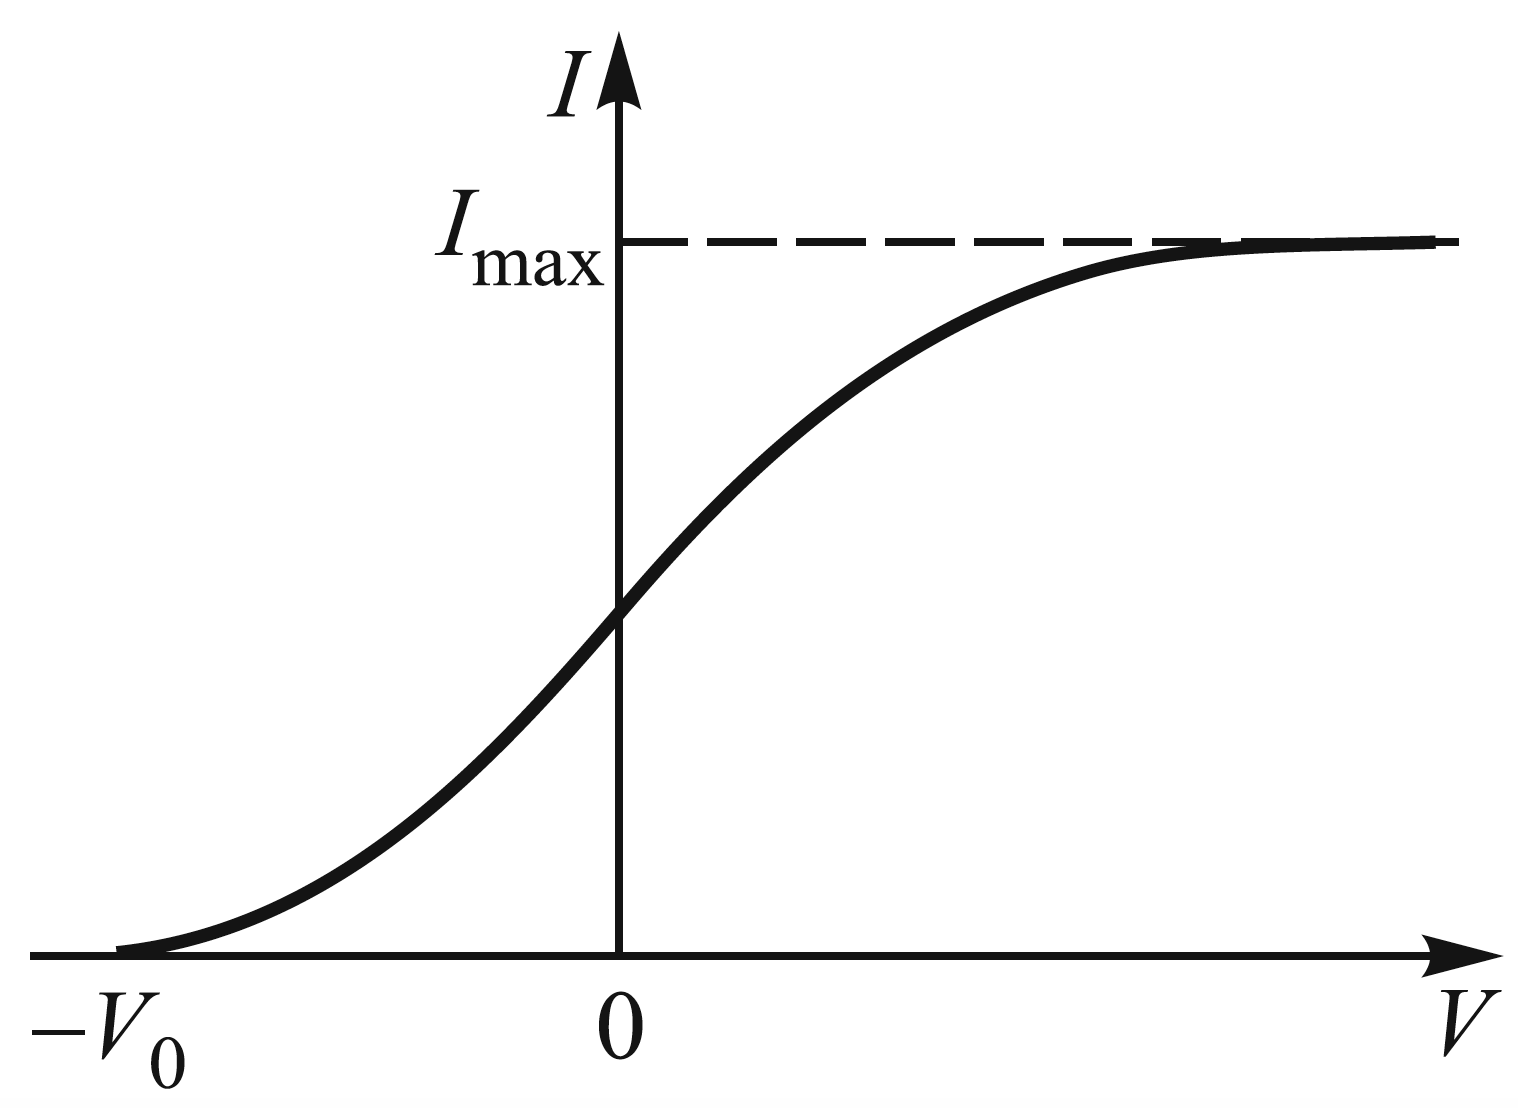
\includegraphics[scale=0.3]{I(V)}
\caption{Зависимость фототока от напряжения на аноде фотоэлемента}
\label{ris I(V)}
\end{figure}
	
Где $ E_{max} $ --  максимальная кинетическая энергия электрона после выхода из фотокатода

$ W $ --- работа выхода электрона из катода (реально энергетический спектр вылетевших из фотокатода электронов непрерывен --- он простирается от нуля до $ E_{max} $)
	
Для измерения энергии вылетевших фотоэлектронов вблизи фотокатода обычно располагается анод, на который подается задерживающий ($ V < 0 $) или ускоряющий ($ V > 0 $) потенциал. При достаточно больших ускоряющих напряжениях фототок достигает насыщения (рис. \ref{ris I(V)}): все испущенные электроны попадают на анод.
	
При задерживающих потенциалах на анод попадают лишь электроны,
обладающие достаточно большой кинетической энергией, в то время как медленно движущиеся электроны заворачиваются полем и возвращаются на катод. При некотором значении $ V = -V_0 $ (потенциал запирания) даже наиболее быстрые фотоэлектроны не могут достичь анода.
	Следовательно, максимальная кинетическая энергия $ E_{max}$ электронов связана с запирающим потенциалом $ V_0 $ соотношением $ E_{max} = eV_0 $. Тогда \eqref{energy balance} примет вид, называемый \textbf{уравнением Эйнштейна}:
	
\begin{equation}
eV_0 = \hbar\omega - W 
\label{Einsteain}
\end{equation}
	
Чтобы определить величину запирающего напряжения, надо правильно экстраполировать получаемую токовую зависимость к нулю, т. е. определить, какова функциональная зависимость $ I(V) $. Расчет для плоского катода, освещаемого светом, и параллельному ему аноду приводит к зависимости
	
\begin{equation}
\sqrt{I} \propto V_0 - V
\label{sqrt I = V}
\end{equation}
	
\textbf{т. е. корень квадратный из фототока линейно зависит от запирающего напряжения}

	В работе изучается зависимость фототока из фотоэлемента от величины задерживающего потенциала $ V $ для различных частот света $ \omega $, лежащих в видимой области спектра. С целью экспериментальной проверки уравнения Эйнштейна определяются потенциалы запирания $ V_0 $ при разных частотах света и строится зависимость $ V_0(\omega) $, которая, как это следует из \eqref{Einsteain}, должна иметь вид
	
\begin{equation}
V_0 (\omega) = \dfrac{\hbar\omega - W}{e}
\label{V(w)}
\end{equation}
	
\begin{figure}[h!]
\centering
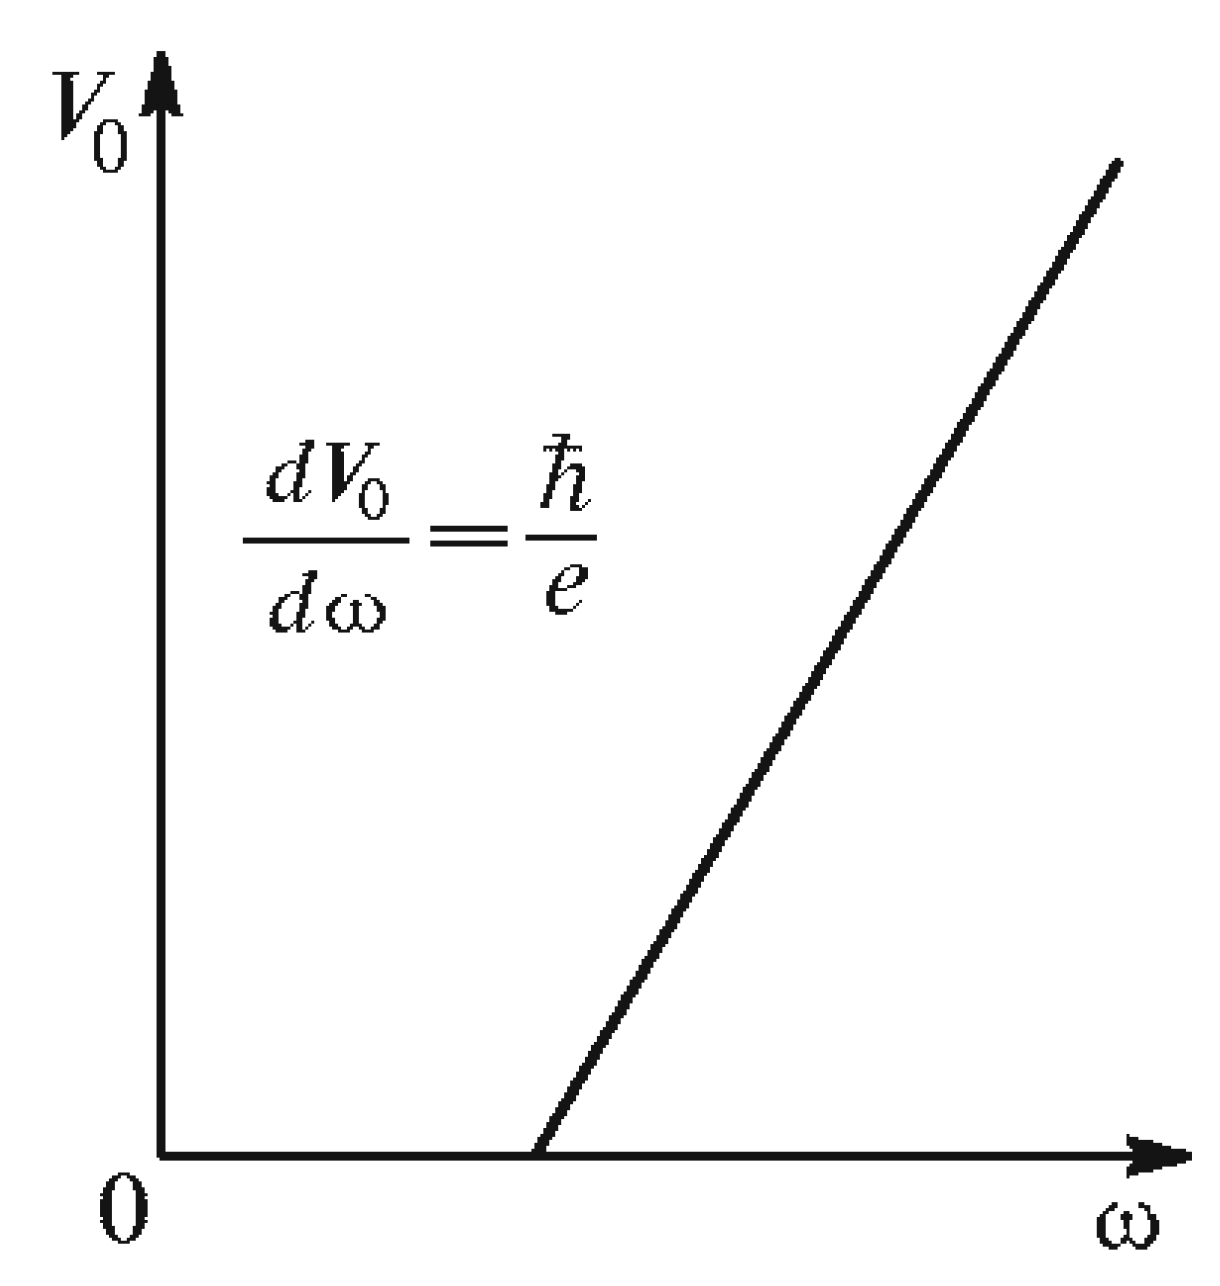
\includegraphics[scale=0.3]{V(w)}
\caption{Зависимость запирающего потенциала
от частоты света}
\label{ris V(w)}
\end{figure}
	
	Потенциал запирания $ V_0 $ для любого катода линейно зависит от
	частоты света $ \omega $. По наклону прямой на графике $ V_0(\omega) $ (рис. \ref{ris V(w)}) можно определить постоянную Планка:
	
	\begin{equation}\label{dV/dw}
	\dfrac{dV_0}{d\omega} = \dfrac{\hbar}{e}
	\end{equation}
	
	Как показывает формула \eqref{dV/dw}, угол наклона прямой $ V_0(\omega) $ не зависит от рода вещества, из которого изготовлен фотокатод. 
\paragraph{Описание установки:}
Принципиальная схема установки представлена на рисунке {\ref{setup}}
\begin{figure}[h!]
\centering
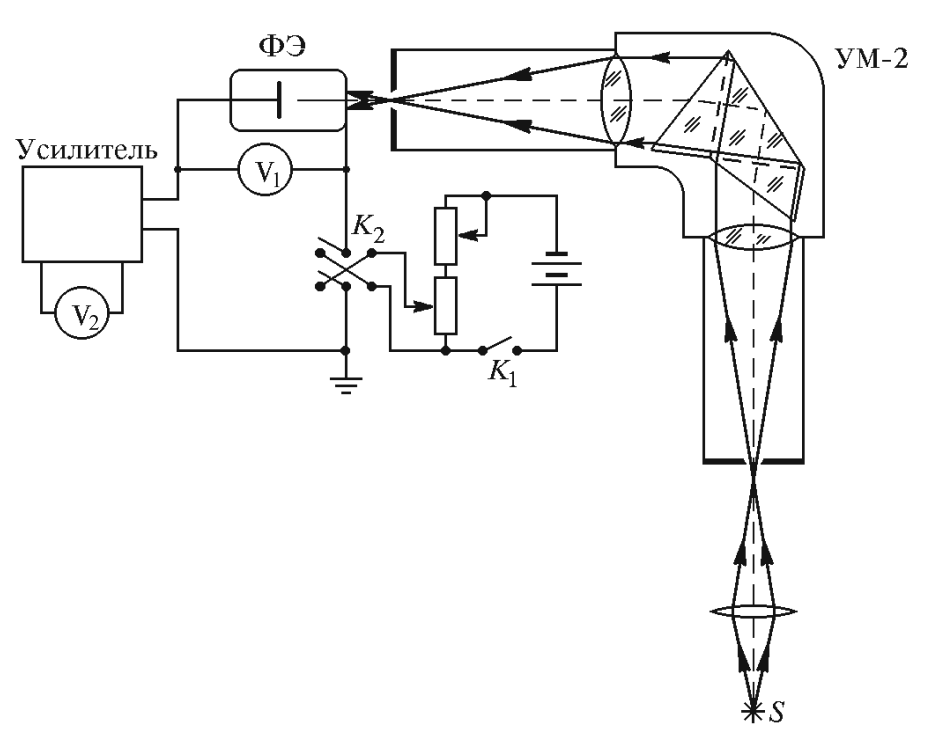
\includegraphics[scale=0.4]{setup.png}
\caption{Принципиальная схема установки}
\label{setup} 
\end{figure}
Установка состоит из:
\begin{enumerate}
\itemsep0em
\item Источника света S (лампа накаливания), свет от которого фокусируется входную на щель с помощью конденсора 
\item Призменного монохроматора УМ-2, выделяющего узкий спектральный интервал
\item Фотоэлемента ФЭ (конструктивно представляет собой откачанный до высокого вакуума стеклянный баллон диаметром 25 мм и высотой 30 мм, внутри которого расположены фотокатод и анод)
\item Усилителя постоянного тока  
\end{enumerate}
\paragraph{Ход работы:}
\begin{enumerate}
\itemsep0em
\item Произведем градуировку монохроматора
\end{enumerate}
\paragraph{Выводы:}
\begin{enumerate}
\item
\end{enumerate}
\end{document}